\section{Bitcoin Blockchain}\label{sec:bitcoin}
Bitcoin was the first cryptocurrency, introduced by an anonymous entity known as Satoshi Nakamoto in 2008.
It is a decentralized digital currency that operates on a peer-to-peer network.
All bitcoin transactions happen on the bitcoin blockchain and after being successfully verified by its
members, they are immutably stored on a block. \cite{BitcoinWhitePaper}

The entities who take part in transactions in the bitcoin network are called wallets.
Nodes may have multiple wallets as well as not have any at all, if they're not interested in participating in
transactions.
\\
Wallets consist of a pair of keys $(K_{\text{priv}}, K_{\text{pub}})$ where:
\begin{itemize}
  \item $K_{\text{priv}}$ uniquely identifies the wallet and is necessary to access the funds of the wallet.
  \item $K_{\text{pub}}$ is a public key which can be generated from the private one.
\end{itemize}

Private keys are hard to memorize and easy to mistype thus, instead of storing the raw private key, users
generate and store it in the form of
a \textit{seed phrase} or \textit{mnemonic} which is a sequence of words that map uniquely to a private key.
The pool of words that can be used is defined in the BIP39 standard.

\subsection{Transactions}
A Bitcoin transaction (TX) is a collection of \textbf{inputs}, \textbf{outputs} and \textbf{metadata} (See
\ref{table:bitcoin_transaction_format}).
Each input in a transaction references the funds of an output of a previous transaction.

As one would expect, the sum of the inputs must not be lower than the sum of the outputs.
This doesn't mean, however, that the two amounts must be equal.
The sum of the inputs must be \textbf{greater or equal} than that of the outputs and is, in practice, always greater.
The difference between the two becomes the transaction fee, rewarded to miners (see the
\hyperref[sec:mining]{\textit{Mining}} section).

An interesting feature of bitcoin transactions is that outputs can't be partially spent.
For example, if a TX output is worth \texttt{10 BTC}, an input of a future transaction referencing it, will
necessarily use the full \texttt{10 BTC}.

It comes naturally to ask how to partially spend funds then.
The answer is simple: if a wallet only wants to send \texttt{2 BTC} but has a unspent output of \texttt{10
BTC}, then the transaction will have:
\begin{itemize}
  \item An input of \texttt{10 BTC} referencing the unspent output.
  \item An output of \texttt{2 BTC} sent to the recipient.
  \item A "change" output of \texttt{8 BTC} sent to the wallet itself.
\end{itemize}

As it appears, wallets \textbf{don't} have a balance in the strict sense. Instead there is the concept of
\textbf{Unspent Transaction Output (UTxO)}.
The \textit{balance} of a wallet be retrieved by inspecting all the transactions within the blockchain and
summing up the UTXOs of the wallet.

\begin{figure}[htbp!]
  \centering
  % Include the image (adjust the file path as needed)
  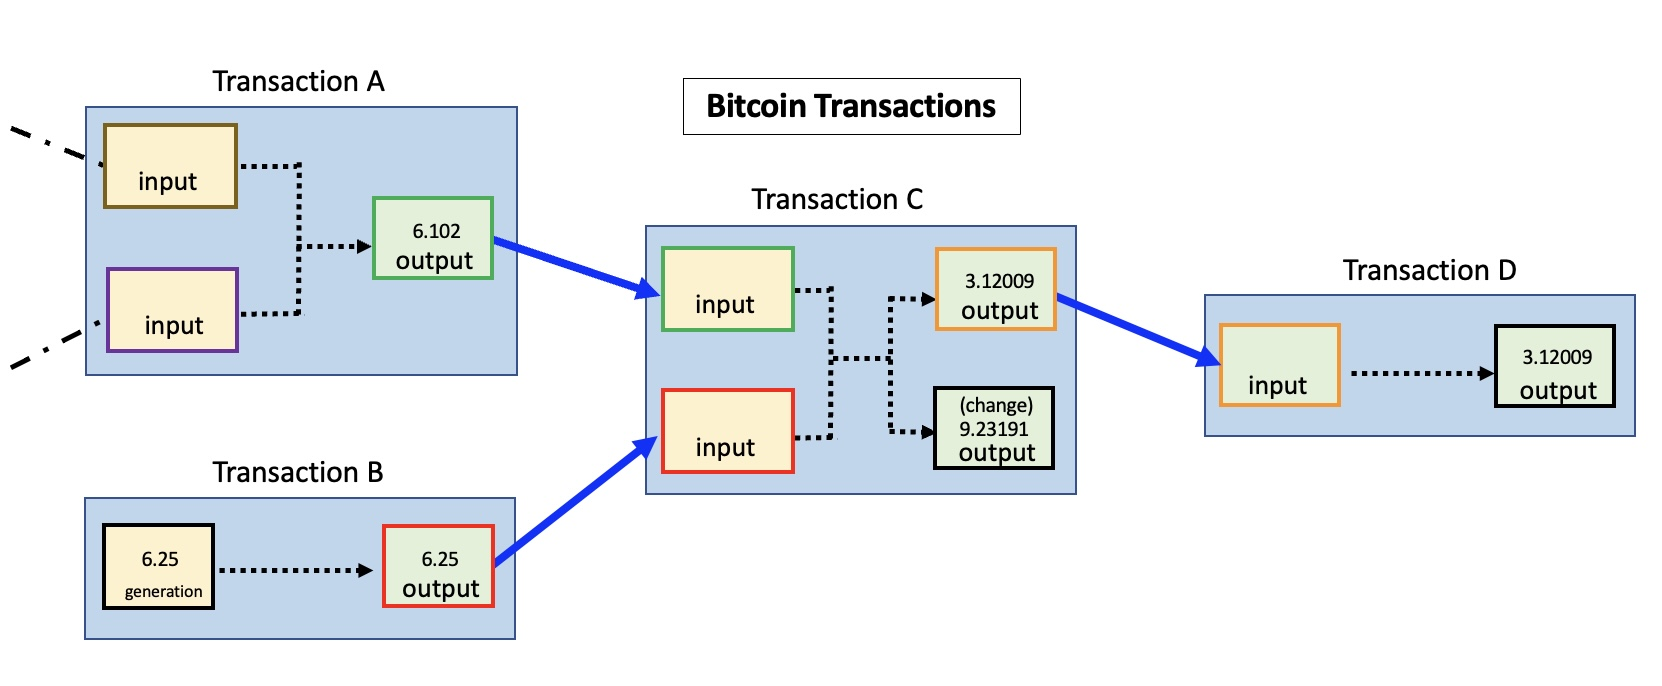
\includegraphics[width=1.0\textwidth]{figures/bitcoin/utxos.jpeg}
  \caption[Bitcoin UTXOs]{Bitcoin Unspent Transaction Outputs (UTxOs): each transaction output is an unspent
  output that can be used as an input in a future transaction.}

  \label{fig:bitcoin_network}
\end{figure}

\begin{table}[H]
  \small
  \centering
  \begin{tabularx}{\textwidth}{|l|X|X|}
    \hline
    \textbf{Field}          & \textbf{Description} & \textbf{Size} \\ \hline
    Version no              & Currently 1. Set to 2 if you use \texttt{OP\_CHECKSEQUENCEVERIFY} to enable
    timelocks & 4 bytes \\ \hline
    Flag                    & If present, always 0001, and indicates the presence of witness data
    & optional 2-byte array               \\ \hline
    In-counter              & positive integer VI = VarInt
    & 1 - 9 bytes                         \\ \hline
    List of inputs          & the first input of the first transaction is also called "coinbase" (its content
    was ignored in earlier versions) & \textless in-counter\textgreater-many inputs \\ \hline
    Out-counter             & positive integer VI = VarInt
    & 1 - 9 bytes                         \\ \hline
    List of outputs         & the outputs of the first transaction spend the mined bitcoins for the block
    & \textless out-counter\textgreater-many outputs \\ \hline
    Witnesses               & A list of witnesses, 1 for each input, omitted if the flag above is missing
    & variable, see Segregated Witness    \\ \hline
    Lock Time               & if non-zero and sequence numbers are \textless 0xFFFFFFFF: block height or
    timestamp when transaction is final & 4 bytes                             \\ \hline
  \end{tabularx}
  \caption{Record format of a Bitcoin transaction (inside a block)}
  \label{table:bitcoin_transaction_format}
  \begin{minipage}{\textwidth}
    \begin{center}
      \footnotesize{Data from \cite{BitcoinWiki} page \url{https://en.bitcoin.it/wiki/Transaction}}
    \end{center}
  \end{minipage}
\end{table}

\subsubsection{Network Communication}
When a wallet intends to transfer funds, the node owning the wallet broadcast the transaction to the Bitcoin network.
The broadcasting happens via \textit{gossip} peer to peer communication. The application level protocol used
for this communication is JSON RPC.
When nodes receive a transaction they do a series of operations:
\begin{enumerate}
  \item They check the transaction's validity: the transaction format is correct, the referenced outputs are
    not already spent and that the wallet has access to them.
  \item They store the transaction by adding it to their \textit{mempool} (a pool of unconfirmed transactions).
  \item They broadcast the transaction to their peers.
\end{enumerate}
On the network, transactions are identified by their \textbf{Transaction ID (TxID)} which is generated by
simply hashing the transaction.
One question which may naturally arise is: when nodes verify transactions, how do they know if a wallet
"owns" the outputs it's trying to spend?
Also how do we identify the recipient of the transaction if the network is anonymous?
To address these questions we must introduce the scripting functionality of the network.

\subsection{Scripting}\label{sec:scripting}
Bitcoin has its own scripting language, called Bitcoin Script, which executes on a stack machine.
Transaction outputs have multiple fields, one of which is the \texttt{script} field, also known as the
\textbf{locking script}.
This locking script specifies the conditions under which the output can be spent.
\begin{table}[htbp!]
  \small
  \centering
  \begin{tabularx}{\textwidth}{|l|X|X|}
    \hline
    \textbf{Field}          & \textbf{Description} & \textbf{Size} \\ \hline
    Value              & Transaction value in satoshis (1 sat = \(10^{-8}\) BTC) & 8 bytes \\ \hline
    Script length     & Positive integer                                          & 1-9 bytes               \\ \hline
    Script              & A calculation which future values need to solve in order to unlock funds & Variable
    \\ \hline
  \end{tabularx}
  \caption{Record format of a TX Output}
  \label{table:bitcoin_output_format}
  \begin{minipage}{\textwidth}
    \begin{center}
      \footnotesize{Data from \cite{BitcoinWiki} page \url{https://en.bitcoin.it/wiki/Transaction#Output}}
    \end{center}
  \end{minipage}
\end{table}

The inputs, in turn, have a field \texttt{scriptSignature}.
In order to verify that the input successfully unlocks the referenced output's funds, the output's
\texttt{script} and the input's \texttt{scriptSignature} are concatenated and executed.
If the execution terminates with \texttt{true} as the only value left in the stack, the transaction is valid.
\subsubsection{Example of Script Execution}
Here's an example of script execution:

\begin{minted}[breaklines,fontsize=\scriptsize]{text}
script = OP_DUP OP_HASH160 <pubKeyHash> OP_EQUALVERIFY OP_CHECKSIG
scriptSig = <sig> <pubKey>
stack = {}

// script = <sig> <pubKey> OP_DUP OP_HASH160 <pubKeyHash> OP_EQUALVERIFY OP_CHECKSIG.
// Push constants to the stack
stack = {<sig>, <pubKey>}
// Execute OP_DUP: duplicate the top of the stack
stack = {<sig>, <pubKey>, <pubKey>}
// Execute OP_HASH160: the constant on top of the stack is hashed.
stack = {<sig>, <pubKey>, <pubKeyHash>}
// Push <pubKeyHash> on top of the stack.
stack = {<sig>, <pubKey>, <pubKeyHash>, <pubKeyHash>}
// Execute OP_EQUALVERIFY: pop the top two values of the stack and check they're equal.
stack = {<sig>, <pubKey>}
// Execute OP_CHECKSIG: pop the top two values of the stack and verify the signature.
stack = {true}
\end{minted}

Bitcoin's scripting language is deliberately non-Turing complete, lacking loops to enhance security
(specifically avoiding DOS attacks on miners).

\begin{table}[htbp!]
  \small
  \centering
  \begin{tabularx}{\textwidth}{|l|X|X|}
    \hline
    \textbf{Field}          & \textbf{Description} & \textbf{Size} \\ \hline
    TxID & Id of the transaction containing the referenced output & 32 bytes \\ \hline
    Output Index & The index within the transaction's outputs array & 4 bytes \\ \hline
    Script length     & Positive integer                                          & 1-9 bytes               \\ \hline
    Script Signature       & A calculation which future values need to solve in order to unlock funds &
    Variable                         \\ \hline
  \end{tabularx}
  \caption{Record format of a TX Input. Note that no value is specified as the value is determined by the
  output being spent}
  \label{table:bitcoin_input_format}
  \begin{minipage}{\textwidth}
    \begin{center}
      \footnotesize{Data from \cite{BitcoinWiki} page \url{https://en.bitcoin.it/wiki/Transaction#Input}}
    \end{center}
  \end{minipage}
\end{table}

\subsection{Anonimity and Addresses}
As the reader may have already noticed from the script example, wallets are identified by their public keys
in transactions.
When two wallet owners agree on a transaction, the receiving wallet generates a public key \(k_{\text{pub}}\)
from its private key \(k_{\text{priv}}\).
From \(k_{\text{pub}}\) a bitcoin address is generated as follows:

\begin{verbatim}
Version = 1 byte of zeros // On the test network, this is 1 byte of ones
Key_hash = Version concated with RIPEMD-160(SHA-256(public key))
Checksum = 1st 4 bytes of SHA-256(SHA-256(Key hash))
Bitcoin Address = Base58Encode(Key_hash concat Checksum)
\end{verbatim}

The payee communicates the address to the payer, who extracts the hash of \(k_{\text{pub}}\) from it and uses
it to create an output with a locking script that basically says:
"Whoever has this public key can access the funds in this output."
When the recipient wants to unlock these funds, they reuse the public key they shared with the payer to craft
an input that successfully those funds.
This mechanism is called \textbf{Pay-to-PubKey-Hash}.

An important thing to note is that, in order to preserve anonimity, a different public key must be used to
generate addresses for distinct transaction.
Otherwise, it would be possible to link the two transactions to the same wallet.

\subsection{Blocks and mining}
For a transaction to be confirmed, it must be included in a \textbf{block}.
Each block is composed of:
\begin{itemize}
  \item \textbf{Header}: Contains metadata (version, timestamp), the previous block's hash, and a
    \textbf{nonce} (used in mining).
  \item \textbf{Body}: Holds transactions in a \textbf{Merkle tree} structure. The root of this tree is
    stored in the block header.
\end{itemize}

The structure of a Merkle tree is shown in \ref{fig:merkle_tree} A merklee tree is chosen
\begin{itemize}
  \item Enables pruning of old transactions.
  \item Allows lightweight nodes to verify transactions with partial tree data.
\end{itemize}

\begin{figure}[htbp!]
  \centering
  % Include the image (adjust the file path as needed)
  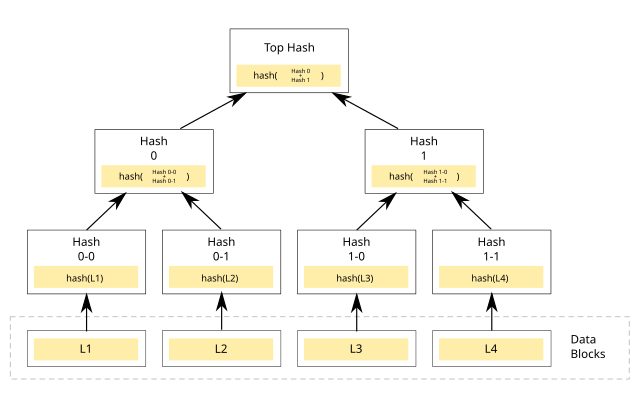
\includegraphics[width=1.0\textwidth]{figures/bitcoin/Hash_Tree.svg.png}
  \caption[Merkle Tree]{Merkle Tree structure: each leaf is a transaction hash, and each internal node is the
  hash of its children.}
  \label{fig:merkle_tree}
\end{figure}
Blocks are crafted by miners, who:
\begin{enumerate}
  \item Gather transactions from the mempool.
  \item Verify them:
    \begin{enumerate}
      \item Check UTxO validity.
      \item Validate scripts (locking/unlocking).
      \item Confirm metadata integrity.
    \end{enumerate}
\end{enumerate}

A block is valid if it satisfies the consensus rules of the blockchain.
This means that its hash satisfies the \textbf{Proof of Work} requirement and that the transactions contained
inside are valid.

\subsubsection{Proof of Work}
As mentioned in \ref{sec:consensus}, proof of work consensus requires solving complex cryptographic puzzles.
In the bitcoin blockchain the puzzle is to find a hash whose numeric value is greater than a network-defined difficulty.
This difficulty is adaptive and is adjusted every 2016 blocks (2 weeks approximately) so as to keep the block
time to around 10 minutes.
Miners adjust the \textbf{nonce} in the block header to find a hash below a network-defined difficulty. This ensures:
\begin{enumerate}
  \item Controlled block production to minimize the chances of forking.
  \item Decentralization by preventing one miner from dominating.
\end{enumerate}

\paragraph{Miner Rewards}
Miners consume a lot of energy and resources to find a Proof of Work so they are rewarded by the network with:
\begin{enumerate}
  \item \textbf{Transaction fees}: Difference between inputs and outputs.
  \item \textbf{Block rewards}: Newly minted Bitcoin (e.g initially \texttt{50 BTC} per block; this amount is
    halved every 210,000 blocks).
\end{enumerate}

\subsubsection{Forks and Consensus}
When two miners create blocks simultaneously, a temporary fork occurs. Miners continue building on the branch
they received first. The chain with more accumulated Proof of Work becomes the canonical chain, and the
shorter branch is discarded.

\subsection{Nodes} \label{sec:bitcoin-nodes}
\textit{"Pure"} nodes of the blockchain are supposed to store all of the blocks somewhere in order to verify
by themselves the integrity of the chian and new blocks.
However, as also noted in the original paper \cite{BitcoinWhitePaper} the blockchain will likely outgrow the
storage capabilities of some nodes at some point.

Thus the proposed solution was to allow for two types of nodes to exist:
\begin{itemize}
  \item \textbf{Full nodes} store the entire blockchain and validate all transactions.
  \item \textbf{Lightweight nodes} store only block headers and query full nodes for details.
\end{itemize}

\subsection{Network protocol}\label{sec:bitcoin-network}
It is worth mentioning how the network layer operates as the implementation we provide in
\ref{chap:implementation} will be similar.
Bitcoin nodes communicate via a peer-to-peer protocol, ensuring decentralized communication between nodes.
Transactions and blocks are propagated using a \textit{gossip protocol}, where nodes relay received data to
their peers. This dissemination ensures redundancy and robustness, even in the presence of node failures.

The messages that can be exchanged by nodes are defined in the Bitcoin wire protocol, which defines the
structures for actions like broadcasting transactions, requesting block data, and maintaining connectivity.
Key message types include:
\begin{itemize}
  \item \textbf{INV (Inventory):} Used to advertise known transactions or blocks.
  \item \textbf{GETDATA:} Requests specific transactions or blocks by their identifiers.
  \item \textbf{BLOCK:} Contains full block data, including headers and transactions.
\end{itemize}

Communication between nodes typically occurs over TCP, with connections initiated via an handshake mechanism:
a version message is exchanged and if both ends accept the other peer's version, they reply with
\textit{verack} messages and the connection is live.
Typically after the handshake is completed, the nodes will use the \textit{addr} and
\textit{getaddr} messages to exchange list of known peers.

Nodes also periodically send \textit{ping} and
\textit{pong} messages to monitor connection health.

To secure the network, transactions are identified by their hashed Transaction ID (TxID), and all data is
verified through cryptographic signatures. The protocol is designed to handle network splits and eventual
consistency, relying on the longest valid chain as the source of truth.
